\chapter{Generting Unit Tests from a UML Activity}
\label{chap:testgeneration}
In this chapter we will present an algorithm that generates unit tests for C-functions from their UML Activity model. The test generation process is divided in fife steps. Between each two steps of our algorithm there is a comprehensive interface defined. Any step can be seen as model to model, model to text, or text to model transformation with the input and output language/model specified. This makes it particularly easy to replace any of the fife steps or extending it with additional features. Thus we are not only specifying one algorithm for generating unit tests from a UML model but also a framework for building further algorithms that generate unit tests from arbitrary input models. If for instance our input model is no more a UML \UMLType{Activity} but a control flow graph specified as instance of any other meta model, then only the first step would need a few changes. In some steps we will even specify different alternatives how to achieve the transformation in this step.\\

Our approach for automated generation of test data is based on mathematical programming and the approach for finding relevant control flow paths is based on a breadth first search with early infeasible path recognition. Alternatively we can also use depth first search.
\section{Generel Overwiew over the Workflow} %BAM DIGGER DIE EINLEITUNG IST GUT!!!
\label{sec:testgenerationOverview}
The transformation from an UML activity to a CPP Unit test code is divided in five steps. Those fife steps are: Normalisation, Rigourous Mathematical programming, Abstract Test Case Generation, Specific Test Data Generation, and finally Unit Test Synthesis. Here we want to give a brief overview over those fife steps. Each of these steps as well as the interfaces between them will be described in detail in the following sections.\\
In a first step, the Normalization (section \ref{sec:Normalization}, we can check some design rules, and parse all embedded OCL constraints, and map only the relevant parts from the UML Model onto a simplified meta model of an activity. The next step is the generation of a mathematical program out of our simplified test model. We are using the AMPL language for specifying a rigorous mathematical program. The third step is a path search where we can find all control flow paths, or those that are necessary to fulfil some coverage criterion of choice. We are considering specific control flow path in an activty test case graph as \emph{abstract test case}. In the fourth step of solving the mathematical program we have each abstract test case encoded as input data for the AMPL model generated during the second step. The AMPL model will be solved by an state of the art solver that works with AMPL. For each abstract test case the solver was able to find valid test data we will store the data in a \emph{test case model}. This test case model will serve as input for the last step. During the unit test synthesis we take the generated solution to the mathematical program and put the values in place within compilable and executable C++ Unit test code. An overview over the complete workflow of our approach is given in figure\ref{fig:workflowOverview}. When infeasible paths need to be detected already during the search of control flow paths the third and fourth step are interfering with each other. How we can determine infeasible sub paths and bound the search for abstract test cases will be explained in the section \ref{sec:EarlyInfeasiblePathRecognition}. Another  feature of the specified algorithm is that we are able to generate boundary values for each abstract test case. For each control flow path in an activity there is a set of input values that will satisfy all constraints along this path and thus is suitable test data for this abstract test case. In testing, bugs are most likely to be triggered when a point at the edge of this set is selected as test data. How we are assuring that a boundary value will be used for testdata generation will be explained in section \ref{sec:boundaryValueSelection}.
\begin{figure}
\includegraphics[width=\textwidth]{pics/workflow.pdf}
\label{fig:workflowOverview}
\caption{Overview over the Unit Test generation workflow}
\end{figure}
%1.Normalize Model, 2.Make model mathematical Rigurous, 3. Search for Control flow Paths. 4 Solve Mathematical Program for the found Control flow Paths to generate specific Input and output Data. 5. Generate Unit Tests
\section{Normalisation}
\label{sec:Normalisation}
\subsection{Design Rules for UML Model} %Structural Design rules
\subsubsection{structural Design Rules}
For our test generation we do assume some design rules to be applied during modelling. The \UMLType{Activity} we generate tests from is an \UMLReference{ownedActivity} of a \UMLType{Class}. The  \UMLType{Class} containing the Activity itself is contained by a \UMLType{Package} or \UMLType{Model}. 
There is an \UMLType{Operation} specifying the \UMLType{Activity}. This \emph{specifying Operation} is either a direct sibling in the UML tree structure and has the same name as the Activity or is explicitly specified by the \UMLReference{specification} reference of the Activity. The specifying Operation will be needed when parsing OCL constraints in section \ref{sec:OCLParsing}.
In figure\ref{fig:StructureExample} we see a tree view of an UML model where those requirements are met.
\begin{figure}
\label{fig:StructureExample}
\includegraphics[width=\textwidht, height=0.5*\textwidth]{}
\caption{Example of a valid structured Model}
\end{figure}
\subsubsection{OCL design rules}
Further we assume that the embedded OCL constraints are either contained within a \UMLType{LiteralString} Element or an \UMLType{OpaqueExpression} with the according Language value set to "OCL". We support a strict subset of the OCL language. The BNF of the supported OCL subset is shown here.

BNF
IntegerLiteral\\
BooleanLiteral: true | false\\
RealLiteral\\
IntVariable\\
RealVariable\\
BoolVariable\\
Number: IntegerLiteral | RealLiteral | IntVariable | RealVariable | ArithmeticOperation\\
ArithmeticOpSymbol: + - * /\\
ArithmeticOperation: Number ArithmeticOpSymbol Number \\
RelationOpSymbol: < | > | <= | >= | = | <> 

RelationOperation: Number RelationOpSymbol Number \\
LogicalOpSymbol: and | or \\
LogicalOperation: Bool LogicalOpSymbol Bool \\

\subsection{A Meta Model suitable for automated Unit Test Generation}
\label{sec:TestCaseGraph}
The developed unit test generation algorithm does not work directly on an UML Model but on an ActivityTestCaseGraph. The ActivityTestCaseGraph contains only those details from the UML Metamodel that are really necessary for the test generation. Since it only contains ready parsed OCL Expressions as abstract syntax trees it is much more suitable for the transformation into a mathematical program. \\
The ActivityTestCaseGraph is defined as an extension of a more general AbstractTestCaseGraph model. The AbstractTestCaseGraph meta model was taylored to fit Activities as well as UML \UMLType{Statemachines} in order to be able to apply algorithms not only to Activities but also to \UMLType{StateMachines} as well as to be able to reuse existing Algorithms from ParTeG for \UMLType{StateMachines} for \UMLType{Activities}.

%????
%Figure \ref{fig:ATCGMetamodel} shows the complete meta model of the ActivityTestCaseGraph including all components from the AbstractTestCaseGraph.
%\begin{figure}
%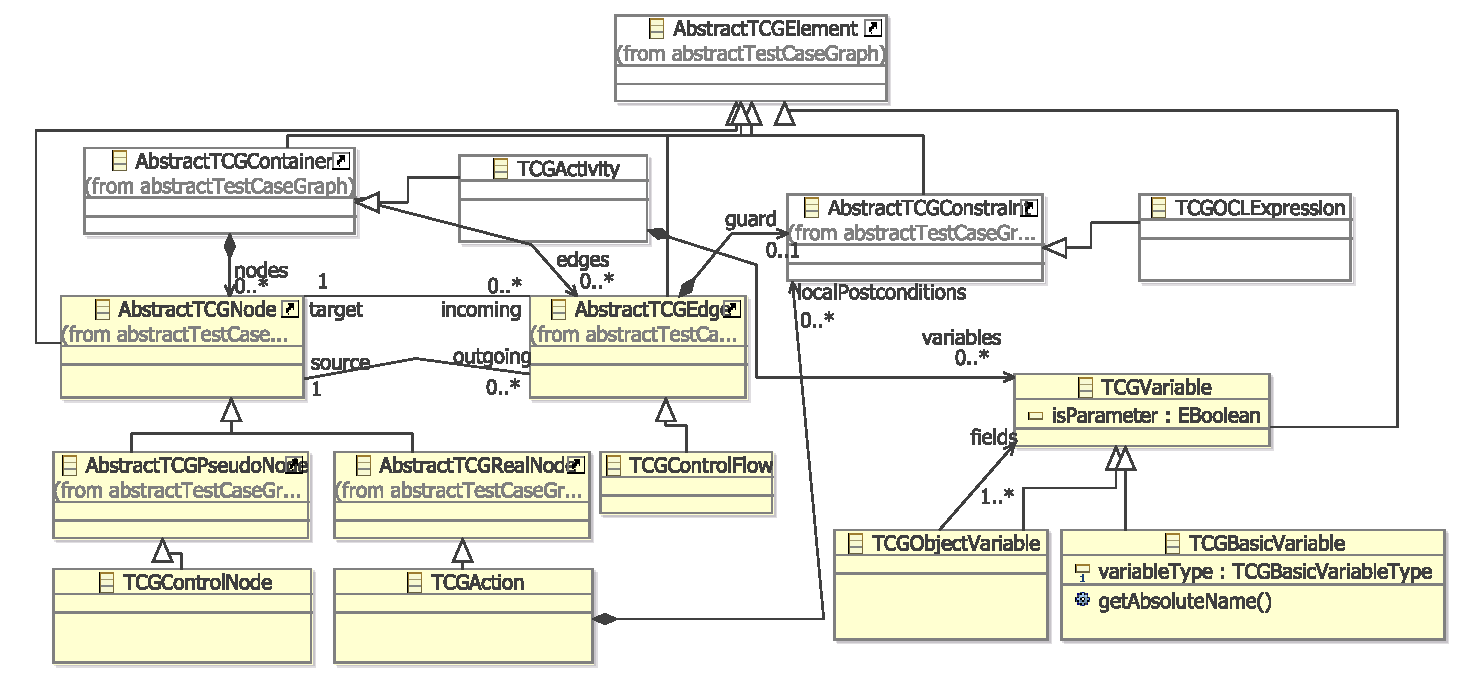
\includegraphics[width=\textwidth]{./pics/ATCGMetamodel.pdf}
%\label{fig:ATCGMetamodel} 
%\caption{Complete meta model of ActivityTestCaseGraph}
%\end{figure}
%????

\subsubsection{Abstract Test Case Graph}

\begin{figure}
\label{fig:AbstractTCGMetaModel}
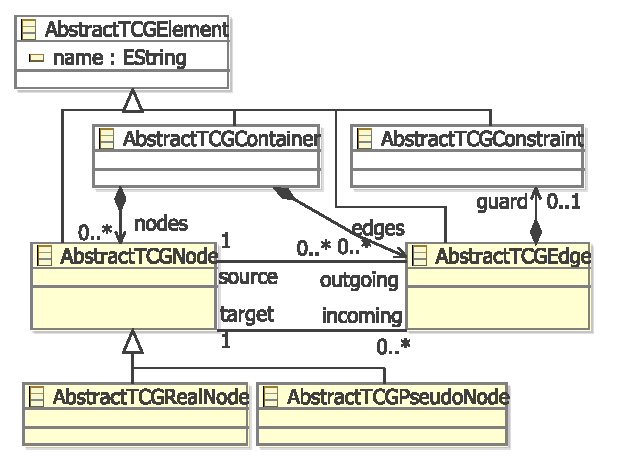
\includegraphics[width=0.5\textwidth]{./pics/AbstractTestCaseGraph.pdf}
\caption{Meta model of the AbstractTestCaseGraph}
\end{figure}
An Abstract Test Case Graph is a directed graph consisting of nodes (AbstractTCGNode) and edges (AbstractTCGEdge). Each edge has source and a target node. Each node can have multiple outgoing and multiple incoming edges.
A node can either be a pseudo node (AbstractTCGPseudoNode) or a real node (AbstractTCGRealNode). A pseudo node is a node that you can insert in the middle of an edge without changing any of the semantics of the test model. Edges can have a guard condition of type AbstractTCGConstraint. Such a graph is contained by a Container (AbstractTCGContainer). The container has a singular reference to one of its owned nodes declaring this as the initial node. \\
The semantics of the activity test case graph is Petri net like. When executing a test case graph we have at the beginning a token in the initial node that can move along the edges. The token can only move along an edge, when its guard condition is true. When a token resides in a node we say that the node is executed.

\subsubsection{Activity Test Case Graph}
\begin{figure}
\label{fig:ActivityTCGMetaModel}
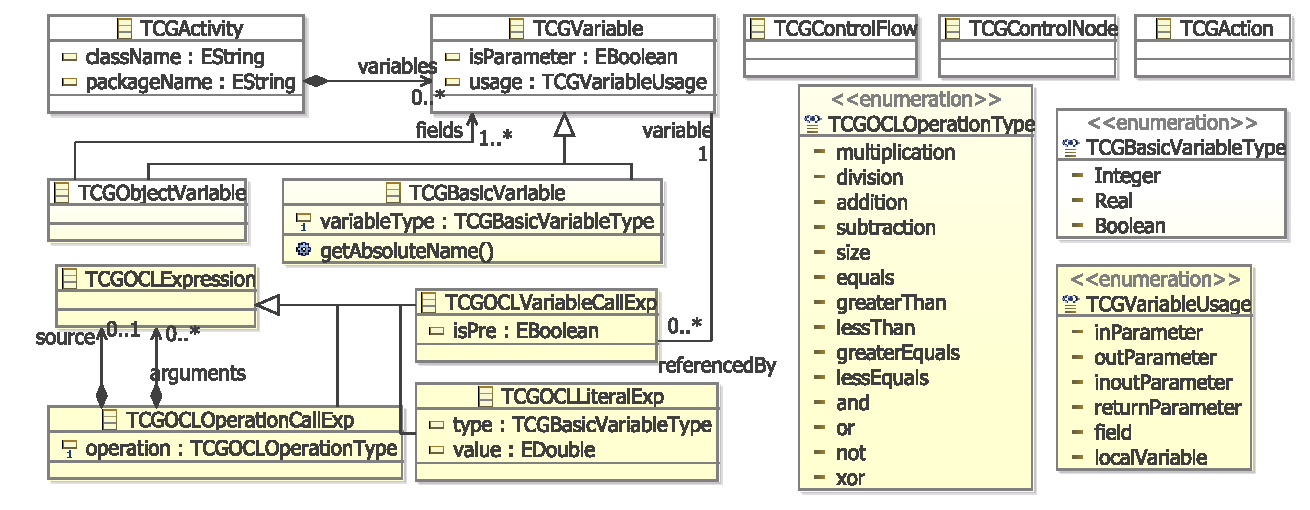
\includegraphics[width=\textwidth]{./pics/ActivityTestCaseGraph.pdf}
\caption{Meta model of the ActivityTestCaseGraph}
\end{figure}
An activity test case graph is an extension to the abstract test case graph especially tailored for test generation from activities. The activity test case graph models control flow and constraints on variables that need to hold at different points during execution of the activity test case graph. Its Metamodel is shown in figure\ref{fig:ActivityTCGMetaModel}.\\
The TCGActivity is an extension of the AbstractTCGContainer. As well as TCGAction, TCGControlNode and TCGControlFlow do refine the types AbstractTCGRealNode, AbstractTCGPseudoNode and AbstractTCGEdge respectively. 
The main extensions to the abstract meta model are the Variables and the elements of an abstract syntax tree to express constraints and the TCGAction.
\paragraph{TCGAction} A TCGAction can in addition to its supertye contain arbitrary many localPostconditions of the type AbstractTCGConstraint. A local Postcondition has the semantic, that it has to be true after the execution of the action. This implies changing some variables throughout the execution of the action.
\paragraph{OCL Abstract Syntax Tree}

TCGOCLExpression is a subtype of AbstractTCGConstraint. A TCGOCLexpression can either be an Operatiton call with a source and  arguments or a TCGOCLLiteralExpression holding a literal value and its data type or a TCGOCLVariableCallExp referencing a TCGVariable. The isPre attribute of TCGOCLVariableCallExp denotes whether in the original OCL expression has been an "@pre" with the token. TCGOCLExpression and its subtypes do form a simplified OCL abstract syntax tree.
\paragraph{Variables}
A TCGVariable can be one of two subtypes either a TCGBasicVariable or a TCGObjectVariable. An object variable is put together by one or more other variables. A basic variable has one of the three variableTypes that can be handled by our approach: Integer, Real, Boolean. A TCGVariable is a place holder for a value. When the isParameter field is true it can only hold one Value throughout the execution of the TCGActivity otherwise it can change its value during each execution of an TCGAction.

\subsection{Transforming UML to ActivityTestCaseGraph}
An Instance of the activity test case graph meta model serves as a normalized input model. We use a model to model transformation to transform an \UMLType{Activity} from a UML Model into an activity test case graph. In many cases the transformation is straight forward: for one Element in the UML model the corresponding element in the activity test case graph is produced. When one element of the UML model is mapped to one Element of the activity test case graph model we call the uml element \emph{source element} and the created element in the activity test case graph model \emph{target element}.
\subsubsection{Mapping UML Elements to Activity Test Case Graph Elements}
\begin{figure}
\label{fig:UML2TCGTranformation}
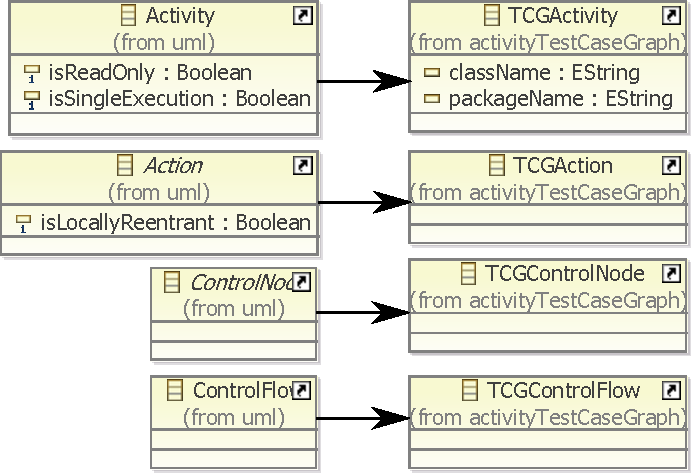
\includegraphics[width=0.6\textwidth]{./pics/UML2TCGTransformation.pdf}
\caption{UML elements being mapped straight forward to activity test case graph elements}
\end{figure}

\paragraph{Activity}
A UML Activity is transformed into a TCGActivity. For the test generation process described in section \ref{sec:UnitTestGen} we need to store the name of the containing class of the Activity as well as the full pathname to the package containig this class in the property fields of the TCGActivity. For each activity all of its ownedNodes as well as ownedEdges are considered for transformation.
\paragraph{Action} Those ownedNodes of the Activity that are a subtype of Action transformed into a TCGAction. To specify the behaviour of the TCGAction localPostconditions are considered for transformation. The detailed semantics of special subtypes of an Action are neglected.
\paragraph{ControlNode}OwnedNodes that are a subtype of ControlNode are transformed into TCGControlNodes. That means they are pseudo nodes. It is assumed that there is only one UML InitialNode. Its corresponding TCGControlNode is referenced by the TCGActivity as initial node.
\paragraph{ControllFlow} Out of the ownedEdges of the \UMLType{Activity} we transform the \UMLType{ControlFlows} into TCGControlFlows. If there is a guard condition this is handled like a constraint.

\subsubsection{parsing OCL Constraints}
\UMLType{Constraints}, and \UMLType{Properties}, as well as \UMLType{Parameters} can not be transformed straight forward. We parse the textual OCL expression contained in a \UMLType{Constraint}, or the \UMLReference{guard} attribute of a \UMLType{ControlFlow}. When the OCL expression was parsed correctly we have an abstract syntax tree of this expression. The elements of this abstract syntax tree will be transformed to TCGOCLExpression elements and all \UMLType{Properties} and \UMLType{Parameters} referenced by the OCL abstract syntax tree will be transformed into TCGVariables. We ensure, that only those OCL expressions are in the activity test case graph that later on can be transformed into an AMPL model as explained in in section \ref{sec:AmplModelling}. We also ensure that our CSP that we will formulate with AMPL will only contain variables that are constraint by at least one constraint. There might be properties of a class that are not changed by an operation and whose value do not have any influence on the control flow in the implementation of this operation. A variable representing such an irrelevant property will not appear in the rigorous model.
\paragraph{Extracting textual OCL}
Textual OCL expressions are contained within \UMLType{Constraints} as explained in section \ref{sec:Constraint}. When the Constraint contains a \UMLType{LiteralString} we will try to parse its \UMLReference{value} as OCL. If the \UMLType{Constraint} contains an \UMLType{Opaque Expression} we will first check whether the \UMLReference{language} attribute contains the value "OCL" and try to parse the corresponding value of the \UMLReference{body} attribute. If the \UMLReference{language} attribute does not contain the value "OCL" then we will try to parse the concatenation of all \UMLReference{body} values of the \UMLType{OpaqueExpression}.\\ The \UMLReference{guard} of a \UMLType{ControlFlow} can also contain a \UMLType{LiteralString} or an \UMLType{OpaqueExpression}. The extraction of textual OCL from a \UMLType{ControlFlow} is analogue to the extraction from a Constraint.
\paragraph{parsing textual OCL}
\label{sec:OCLParsing}
Details of the OCL have been explained in \ref{sec:Constraint}. For this thesis we consider three types of constraints: \emph{invariants}, \emph{postconditions} and \emph{guard conditions}. Every OCL constraint is parsed with respect to a \emph{context}. The context resolves the variables referenced within the OCL expression. For Example the "self" keyword always returns the instance for which the constraint is evaluated.\\
Textual OCL found inside a \UMLType{Constraint} contained by the \UMLReference{ownedRule} reference of either the \UMLType{Activity} or its containing \UMLType{Class} will be interpreted as invariant. Invariants need to be true before the \UMLType{Activity} is executed, throughout its execution, and after the execution of the \UMLType{Activity} has finished. We are parsing the invariants according to the OCL specification as invariants of the specifying \UMLType{Operation}. \\
The OCL expressions found within \UMLReference{guards} of \UMLType{ControllFlows} will also be parsed as if they were an invariant of the specifying \UMLType{Operation}.
That means for guards and invariants all attributes of the \UMLType{Class} as well as all \UMLReference{ownedParameters} of the specifying \UMLType{Operation}, and all properties of the containing \UMLType{Packages} are accessible.\\
\UMLType{Actions} can also contain multiple \UMLType{Constraints} within their \UMLReference{localPostcondition} reference. Any textual OCL found within a \UMLReference{localPostcondition} will be parsed as postcondition in the context of the specifying \UMLType{Operation}. All variables accessible for guards and invariants are also accessible for postconditions. Only in postconditions the OCL "@pre" is allowed. Postconditions are required to hold after the execution of the \UMLType{Action} they belong to. With "@pre" we refer to the value of a variable before the execution of the \UMLType{Action}.

\paragraph{Transforming the Abstract Syntax Tree}
\begin{figure}
\includegraphics[width=\textwidth]{}
\end{figure}
If the OCL parser was supplied with a valid OCL expression for the context that was assumed then it will return an abstract syntax tree for the parsed OCL expression. We are interested in a subset of the OCL abstract syntax trees namely the subset presented in section \ref{sec:OCL}. \\
Boolean literals, integer literals and unlimited real literals will all be transformed into a TCGOCLLiteralExp the it value is stored as a double precision floating point format. The type attribute of the target element is set according to whether the source element was a boolean literal, integer literal or a unlimited real literal. For the type boolean $0.0$ expresses a false literal and $1.0$ expresses a true literal.\\
Parameter call expressions and variable call expressions are transformed into TCGOCLVariableCallExp elements. If the original OCL token was tagged with an "@pre" then the isPre attribute is set to true. Each property call expression will have a reference to a \UMLType{Property} and each variable call expression will have a reference to a \UMLType{Parameter} those referenced elements will be transformed into TCGVariables as explained in the next paragraph. The target TCGOCLVariableCallExp will get a reference to the target TCGVariable.\\
An OCL abstract syntax tree may also contain operation call expressions. Each operation call expression will be transformed into a TCGOCLOperationCallExp. The attribute operation will be determined from the name attribute of the operation referenced from the source element. If the operations name is "=" then the targets operation is set to equals, if the sources operation name is "*" then the targets operation is multiplication and so on. An operation call exp has a source and arguments those elements are also transformed to TCGOCLExpressions and the transformed elements are added to the targets source and arguments references.\\
Every root TCGOCLExpression directly contained by a TCGAction, TCGControlFlow, or TCGActivity gets its name property set. The transformation ensures that every root TCGOCLConstraint has a globally unique name. In the original UML model it is not the case that each \UMLType{Constraint} has a globally unique name.

\paragraph{transforming Properties and Parameters}
whenever the OCL abstract syntax tree containes a property call or a variable reference then the referenced \UMLType{Property} or \UMLType{Parameter} will be transformed into a TCGVariable. All TCGVariables are contained by the variables reference of the root element of the activity graph, the TCGActivity.\\
For \UMLType{Parameters} and \UMLType{Properties} we need to check their \UMLReference{type} reference. If the name of the \UMLType{Type} is one out of a list of names that can be mapped to either Integer, Real or Boolean then a TCGBasicVariable is created for it and its variableType field set accordingly to one out of Integer, Real or Boolean. The exact mapping of names of the \UMLType{Type} to a TCGvariableType is implementation specific. One could for example map from "uint32\_ t" to Integer.\\
If a \UMLType{Parameter} was transformed into a TCGBasicVariable then the isParameter field is set to true, indicating that this Variable has been a \UMLType{Parameter}. For \UMLType{Properties} the isParameter field of the resulting TCGBasicVariable will be set to false.\\
The field usage of the the TCGBasicVariable can take values from the enumeration TCGVariableUsage. This information will be needed when creating the c or c++ unit tests as described in section \ref{sec:UnitTestGeneration}. If the TCGBasicVariable was created to represent a Parameter it could have been an input parameter, an output parameter, an inout parameter, or a return parameter. The value of the usage field for a transformed \UMLType{Parameter} is determined by the value of the \UMLReference{direction} field of the original \UMLType{Parameter}.\\


%according to the OCL specification as explained in section \ref{sec:OCL}. 

% When the textual expression was successfully parsed according to the OCL specification we hold an abstract syntax tree of the OCL Expression as explained in \ref{sec:OCL}. The elements from the OCL abstract syntax tree are then transformed into TCGOCLExpressions. Whenever a 
%transform then only those \UMLType{Properties} and \UMLType{Parameters} into TCGVariables, that are referenced in the parsed OCL Expressions.\\ 

%A UML Constraint can be specified in several ways e.g as StringLiteral or as OpaqueExpression. It is depending on the used modelling tool how the textual OCL is saved in the Model. We are extracting the textual OCL Expressions and parse them according to the OCL specifications. If they can not be parsed the extracted text was either not an OCL expression or it is a faulty one. In those cases this constraint will be ignored.


\subsection{Further Model 2 Model Transformations}
After 

\subsubsection{Removing logical operations}

%\subsubsection{
\subsubsection{Handling Structured Activity Nodes}
\subsubsection{Mapping self defined Datatypes to standard Types}
Explain the ActivityTestCaseGraph Metamodel and the transformation from UML with embedded OCL to it. 
suggest a few further M2M transformations to make the model easier to digest for the actual test generation.
\subsubsection{Adding Continuity Constraints}
From imperative programming we are used that, if nothing is specified nothing will happen. It is especially important that x will not take a new value during a computation if we do not explicitly state an assignment for x. In OCL there is nothing like an assignment. In OCL we are expressing constraints telling us which assignment would be legal and which not. If for a specific variable $x$ there is no constraint referring to it that means, that this variable can take any value. Consequently the user needs to make it explicit when a variable shall not be changed during the execution of an \UMLType{Action}. The user can state that a variable $x$ shall stay unchanged by adding a \emph{continuity constraint} to the \UMLReference{localPostconditions} of each \UMLType{Action} that shall not change the variable. The continuity constraint will contain the textual OCL "x=x@pre". That means x shall have the same value as x had before the execution of this \UMLType{Action}.\\
We can support the user by adding a large amount of continuity constraints automatically. All variables that are not constrained at all within the postconditions of an action will have the same value after execution of the Action as before. We need to determine the set difference between the set of all variables in the TCGActivity and the set of all free variables referenced from the local postconditions for each action within the activity. The difference of those sets is the set of variables, that need a continuity constraint to prevent the constraint solver from setting them to completely arbitrary values. The Algorithm for adding continuity constraints is given in figure \ref{fig:ContinuitConstraintAlgorithm}.
\begin{figure}\label{fig:ContinuitConstraintAlgorithm}
\begin{verbatim}
Vars = set of all Variables contained by the TCGActivity
for each TCGAction in TCGActivity
	S = {} /* set of referenced free variables
	for each TCGOCLConstraint in localPostconditions
		visit all nodes and whenever a free variable is found ad it to S
	end
	C = Vars\ S
	add a continuity constraint for each variable in C to the current TCGAction.
end
end
\end{verbatim}
\end{figure}
\section{AMPL Modeling}
\label{sec:atcg2Ampl}
In the last section we have extracted all necessary information from a UML model and stored it in a normalized way in an activity test case graph model. All OCL expressions have been parsed and a simplified version of the abstract syntax tree is incorporated in the activity test case graph model. For the next steps we will exclusively work with this normalised test model as a source model and no more access the original UML model.\\
In this step we will perform a model to text transformation from an activity test case graph to an AMPL model. We explained the AMPL mathematical programming language in section \ref{sec:AMPL}. In order to make the model executable we need a rigorous mathematical representation for it. In many cases a higher order logic with quantifiers is used to make OCL specifications rigorous and executable \cite{krieger2008executingUnderspecifiedOCL},\cite{brucker2012theoremProverBasedTesting}. We will use a mathematical and mixed integer programming approach to make the activity test case graph executable.\\
\subsection{How to Transform an Activity Test Case Graph into a Mathematical Program}
The mathematical program in AMPL consists of two parts the model and the data. When we want to generate suitable test data for a certain path within an activity test case graph we need an AMPL model and the corresponding AMPL data. An AMPL model encodes a complete activity test case graph including all variables and all constraints that are contained. The control flow path within this activity test case graph needs to be encoded in the AMPL data part. How this exactly is done will be explained throughout this chapter.\\
\begin{figure}
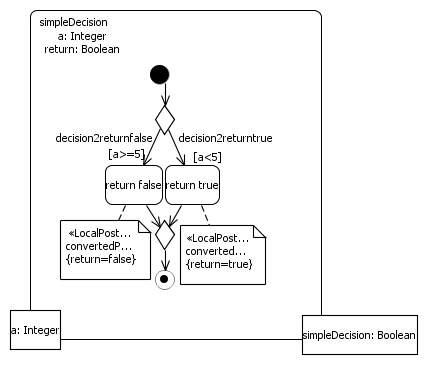
\includegraphics[width=0.5\textwidth]{./pics/SomeActivityDiagrams.png}
\end{figure}
During the execution of an activity test case graph we have an initial state where every variable has a specified value. A state is specified by the complete value assignment for all variables. After each execution of an action this state might change according to the rules given in the actions postconditions. Postconditions can specify a relation between the value assignment in the current state and a value assignment in the previous state. The states are interconnected with each other via postconditions. The set of all postconditions can be seen as a state transition function. In order to traverse a control flow edge its guard needs to evaluate to true in the current state. Guard conditions can only specify relations between the value assignments within a single state.\\ 
The AMPL model models the execution of an activity as a series of states. All postconditions and guards are contained in the model as constraints, that can be switched on and off for each state within the series of states. For example if we assume an activity modelling the statement \begin{verbatim}if (x<5) then y=x else y=x-100 \end{verbatim} that would look like depicted in figure \ref{fig:ActivityExample}. There are two possible paths. Each path contains exactly one action. Consequently we need two states: one initial state and one state after the execution of the first action. We have two variables $x$ and $y$. For each variable we need in AMPL an array of length 2 in order to hold the value assignment for those variables in each state. We will denote the value assignment for $x$ in the i-th state as $x_i$. Lets assume we want to generate test data for the \texttt{then} path. In this case in the first state the constraint $x_1<5$ is activated and in the second state we have the constraint $x_2=x_1$ activated. Further in section \ref{sec:UML2atcg} the constraint $x_1=x_2$ would have been introduced since there is no other rule constraining $x_2$, and whenever a value is unconstrained we want to preserve the variables value from the previous state. The resulting problem is an linear program with 4 unknown values and 3 linear equations and inequations. The value of $y_1$ will stay completely unconstrained, since there is no previous state before the first and initial state.\\
%Any variable can be either an integer, a real number or a boolean. Each postcondition, guard condition and invariant will show up as constraint in the AMPL model. In the data to the model we will specify which constraints are activated for which states.  We can also see the set of postconditions as a state transition function. \\
We will start with the transformation of the variables into ampl variables and then transform guards and postconditions into AMPL constraints. Each AMPL model has one parameter called \texttt{pathlength} representing the number of actions on a path. For each action with postconditions, and each control flow with a guard there is one set that is required to be a subset of $[1..pathlength]$ specifying these states, in which those constraints are active. We will call them \emph{activation sets}. The value of the parameter \texttt{pathlength} as well as the elements of each activation set will be specified in the input data to the AMPL model. In this way there is one AMPL model per activity and any path we want to generate test data for can be specified via the data to the AMPL model.\\

The built AMPL model will be synthesised according to the following form:
\begin{verbatim}
AMPLModel: "param pathlength;"
(VariableDeclarations)*
(ActionPostconditionConstraints)*
(ControlFlowGuardConstraints)*
\end{verbatim}
For each variable in the source model there will be one VariableDeclaration token, for each Action there will be one ActionPostconditionConstraints token. And for each control flow having a guard condition there will be a ControlFlowGuardConstraints token. The synthesis of these tokens will be explained in more detail in the respective subsections on \ref{sec:Variables2AMPL}, \ref{sec:Postconditions2AMPL}, and \ref{sec:Guards2AMPL}.



%Tell about the AMPL Modelling i.e. variables are becoming arrays to hold one initial Value and for each TCGAction on the Path one that makes its postconditions and general Invariants valid. One specific control flow Path is encoded in the AMPL data, so we can take advantage of the interactive solving capabilities of AMPL and the connected solvers.
\subsection{Transforming TCGVariables}
\label{sec:Variables2AMPL}
Every variable has one out of three possible types: integer, real and boolean. In AMPL if nothing else is specified an AMPL variable is interpreted as a variable in the domain of real numbers. AMPL also natively supports variables in the domain of integers. For integer variables we always need an upper and a lower bound that will be set to $+10000$ and $-10000$ by default. Without these bounds we have experienced some problems with Ampl and its solvers this will be explained more detailed in \ref{sec:LimitationsAMPL}. The boolean domain is modelled as the set $ \left\lbrace 0 , 1 \right\rbrace $, where 0 corresponds to false.\\
Since every variable can have different values in each state of the execution each variable will in AMPL be modelled as an variable array of fixed size. The size of the the array is defined as the \texttt{pathlength}. When the isParameter attribute of the TCGVariable is true then the variable is constant and cannot change its value from one state to another, thus we can model those variables as a single AMPL variable.\\
The BNF of the synthesised code is given as follows. \texttt{variableName} is the unique name of the source TCGVariable.
\begin{verbatim}
VariableDeclaration: "var "(variableName)("{0..pathlenth}")? (TypeSpecification) ":=1;"
TypeSpecification: ((Integer) | (Real) | (Boolean))
Integer: ": integer >=-10000, <= 10000"
Real: ">=-10000, <= 10000"
Boolean: " in 0..1"
\end{verbatim}

\subsection{Transforming LocalPostConditions}
\label{sec:Postconditions2AMPL}
For each TCGAction the activation set is declared as a subset of $\left[0..\texttt{pathlength}\right]$ in the AMPL model. The name of the activation set is the name of the TCGAction. The name of each TCGAction is guaranteed to be unique within one activity test case graph model. Each local postcondition of a TCGAction is transformed into an indexed collection of constraints over this activation set. 

\subsection{Transforming Guards}
\label{sec:Guards2AMPL}
The transformation of guards works analog to local postconditions.

\subsection{Specifying Control Flow Paths in the AMPL Data}
\subsection{Generate Boundary Values}
\section{Pathsearch}
\label{sec:pathsearch}
Bounded BFS, and Bounded DFS, and DFS with early infeasible Path elimination.
Suggest to extend the search algorithms to work with test goals as explained by Stephan Weißleder.
\subsection{Depth First Search}
\subsection{Breadth First Search}
\subsection{Early Infeasible Path Elimination}
This feature can also be used to specify for loops an upper bound of iterations as well as a lower bound of loop iterations to test. You just need to add some guard conditions in front of the loop referencing the loop variant.
\section{solving}
\label{sec:testgenerationSolving}
By adding an objective function to the AMPL Model after any solution has been found it is possible to get boundary values for testing.

\section{Unit Test Synthesis}
\label{sec:testgenerationUnitTestSynthesis}

\section{Implementation}
\label{sec:testgenerationImplementation}
say a few words about EMF and Eclipse Plugin. Tell that I used Eclipse org.eclipse.ocl.uml and eclipse org.eclipse.uml2.uml packages. 
\subsection{The Eclipse Modelling Framework}
\cite{EMF}
\subsubsection{Importing Models from Atego Artisan Studio}
\subsubsection{Model transformations}
\subsubsection{Parsing OCL Expressions}
\subsection{Using the resulting Plugin}
